\documentclass[aspectratio=169,11pt]{beamer}
% ==========================================================================
%  KSA lecture-slide theme  =  stock beamer "Boadilla"  +  KSA colour theme
%  brand colours sampled from the official KSA symbol mark:
%    Deep Prussian Blue  #2E3192   (지성 - intellect)
%    Golden Gray         #D6CBB1   (감성 - sensibility)
%  Engine: XeLaTeX.  Usage:
%    \documentclass[aspectratio=169,11pt]{beamer}
%    \input{../../theme/ksa-theme.tex}
%  Each deck lives in its own slides/kor/<deck>/ folder together with its
%  own images; ../../figs/ is kept only as a fallback for the shared cache.
% ==========================================================================

\usepackage{fontspec}
\usepackage{amsmath,amssymb}
\usepackage{graphicx}
\graphicspath{{figs/}{./}{../../../figs/}}
\usepackage{booktabs}
\usepackage{listings}
\usepackage{varwidth}

% ---- fonts (no ctex/xeCJK on this box -> fontspec drives CJK directly) -----
\defaultfontfeatures{Ligatures=TeX}
\setmainfont{Noto Sans CJK KR}
\setsansfont{Noto Sans CJK KR}
\setmonofont{Noto Sans Mono CJK KR}[Scale=0.92]

% ---- base theme: stock Boadilla ------------------------------------------
\usetheme{Boadilla}
\usefonttheme{professionalfonts}
\setbeamertemplate{navigation symbols}{}

% ---- KSA colour theme (recolour the stock theme) --------------------------
\definecolor{ksablue}{HTML}{2E3192}
\definecolor{ksabluedk}{HTML}{20226A}
\definecolor{ksagold}{HTML}{D6CBB1}
\definecolor{ksagolddk}{HTML}{A9976B}
\definecolor{ksared}{HTML}{C0392B}
\definecolor{ksagray}{HTML}{5B5B5B}

\setbeamercolor{structure}{fg=ksablue}
\setbeamercolor{alerted text}{fg=ksared}

\setbeamercolor{palette primary}{fg=white,           bg=ksablue}
\setbeamercolor{palette secondary}{fg=white,         bg=ksablue!85!black}
\setbeamercolor{palette tertiary}{fg=white,          bg=ksabluedk}
\setbeamercolor{titlelike}{fg=ksablue}
\setbeamercolor{frametitle}{fg=ksablue,bg=}
\setbeamercolor{title}{fg=ksablue}
\setbeamercolor{author}{fg=ksagray}
\setbeamercolor{institute}{fg=ksagray}
\setbeamercolor{block title}{fg=white,bg=ksablue}
\setbeamercolor{block body}{fg=black!85,bg=ksablue!6}
\setbeamercolor{item}{fg=ksablue}
\setbeamercolor{section in toc}{fg=black!85}

\setbeamerfont{frametitle}{series=\bfseries}
\setbeamerfont{title}{series=\bfseries}

% ---- footline:  KSA mark | "Made by ..." | n / N   (matches reference) ----
\newcommand{\ksacredit}{}
\setbeamertemplate{footline}{%
  \hbox{%
    \begin{beamercolorbox}[wd=.18\paperwidth,ht=2.6ex,dp=1.5ex,leftskip=1.1em]{}%
      \raisebox{-0.35ex}{\includegraphics[height=2.0ex]{ksa-logo.png}}%
    \end{beamercolorbox}%
    \begin{beamercolorbox}[wd=.64\paperwidth,ht=2.6ex,dp=1.5ex,center]{}%
      {\scriptsize\color{ksagray}\ksacredit}%
    \end{beamercolorbox}%
    \begin{beamercolorbox}[wd=.18\paperwidth,ht=2.6ex,dp=1.5ex,rightskip=1.1em]{}%
      \hfill{\scriptsize\color{ksablue}\insertframenumber\,/\,\inserttotalframenumber}%
    \end{beamercolorbox}%
  }%
  \vskip2pt
}

% ---- section divider: stock \sectionpage, KSA-coloured -------------------
\setbeamertemplate{section page}{%
  \begingroup\centering
    {\color{ksagolddk}\rule{0.16\paperwidth}{1pt}}\par\vskip1.0em
    {\usebeamerfont{title}\color{ksablue}\insertsectionhead\par}\vskip1.0em
    {\color{ksagolddk}\rule{0.16\paperwidth}{1pt}}\par
  \endgroup
}
\AtBeginSection[]{\begin{frame}[plain,noframenumbering]\vfill\sectionpage\vfill\end{frame}}

% ---- code listings ------------------------------------------------------------
\lstdefinestyle{ksa}{%
  basicstyle=\ttfamily\scriptsize,
  keywordstyle=\color{ksablue}\bfseries,
  commentstyle=\color{ksagray}\itshape,
  stringstyle=\color{ksagolddk},
  numberstyle=\tiny\color{ksagray},
  backgroundcolor=\color{ksablue!6},
  frame=leftline, framerule=1.4pt, rulecolor=\color{ksablue},
  xleftmargin=1em, aboveskip=0.8em, belowskip=0.4em,
  showstringspaces=false, breaklines=true, language=Python,
}
\lstset{style=ksa}

% ---- handy macros -----------------------------------------------------------
\newcommand{\kb}[1]{\textbf{\color{ksablue}#1}}   % blue keyword
\newcommand{\kq}[1]{\textbf{\color{ksared}#1}}    % red key-question

\setbeamerfont{title}{series=\bfseries,size=\fontsize{24}{30}\selectfont}
\setbeamerfont{subtitle}{series=\bfseries,size=\fontsize{14}{18}\selectfont}
\setbeamerfont{author}{size=\normalsize}
\setbeamerfont{institute}{size=\small}
\graphicspath{{figs/}{../../../../assets/}}
\makeatletter
\newcommand{\markpage}[1]{\protected@write\@auxout{}{\string\newlabel{#1}{{\the\c@framenumber}{}}}\hypertarget{#1}{}}
\newcommand{\pref}[1]{\hyperlink{#1}{\textcolor{ksagolddk}{(p.\ref{#1})}}}
\makeatother

\renewcommand{\ksacredit}{Machine Learning 1 \,\textperiodcentered\, 데이터 증강}
\title{데이터 증강 (Data Augmentation)}
\subtitle{뜻은 그대로, 모양만 바꿔 데이터를 늘린다}
\author{Machine Learning 1}
\institute{한국과학영재학교 (KSA)}
\date{}
\begin{document}
\begin{frame}[plain,noframenumbering]\titlepage\end{frame}

% --- 오늘의 질문
\begin{frame}{오늘의 질문}
\vfill
\centering
{\LARGE 고양이 사진이 딱 \textbf{1장}}\\[0.6em]
{\LARGE 이걸로 학습 데이터 \kq{10장}을 만들 수 있을까?}\\[1.2em]
{\large 데이터를 더 모으기는 비싸다 \quad 가진 데이터를 \textbf{더 쓸모 있게} 쓸 수 없을까?}
\vfill
\note{고양이 사진이 딱 한 장 있습니다. 이걸로 학습 데이터 열 장을 만들 수 있을까요? 지금까지 과대적합을 막는 가장 확실한 방법은 데이터를 더 모으는 것이라고 했습니다. 하지만 사진을 찍고 정답을 붙이는 데는 돈과 시간이 듭니다. 오늘은 가진 데이터를 조금씩 바꿔 새 학습 데이터로 쓰는 방법, 데이터 증강을 배웁니다.}
\end{frame}

% --- 고양이
\begin{frame}{가진 사진을 조금씩 바꾼다}
\markpage{cats}
\vfill
\centering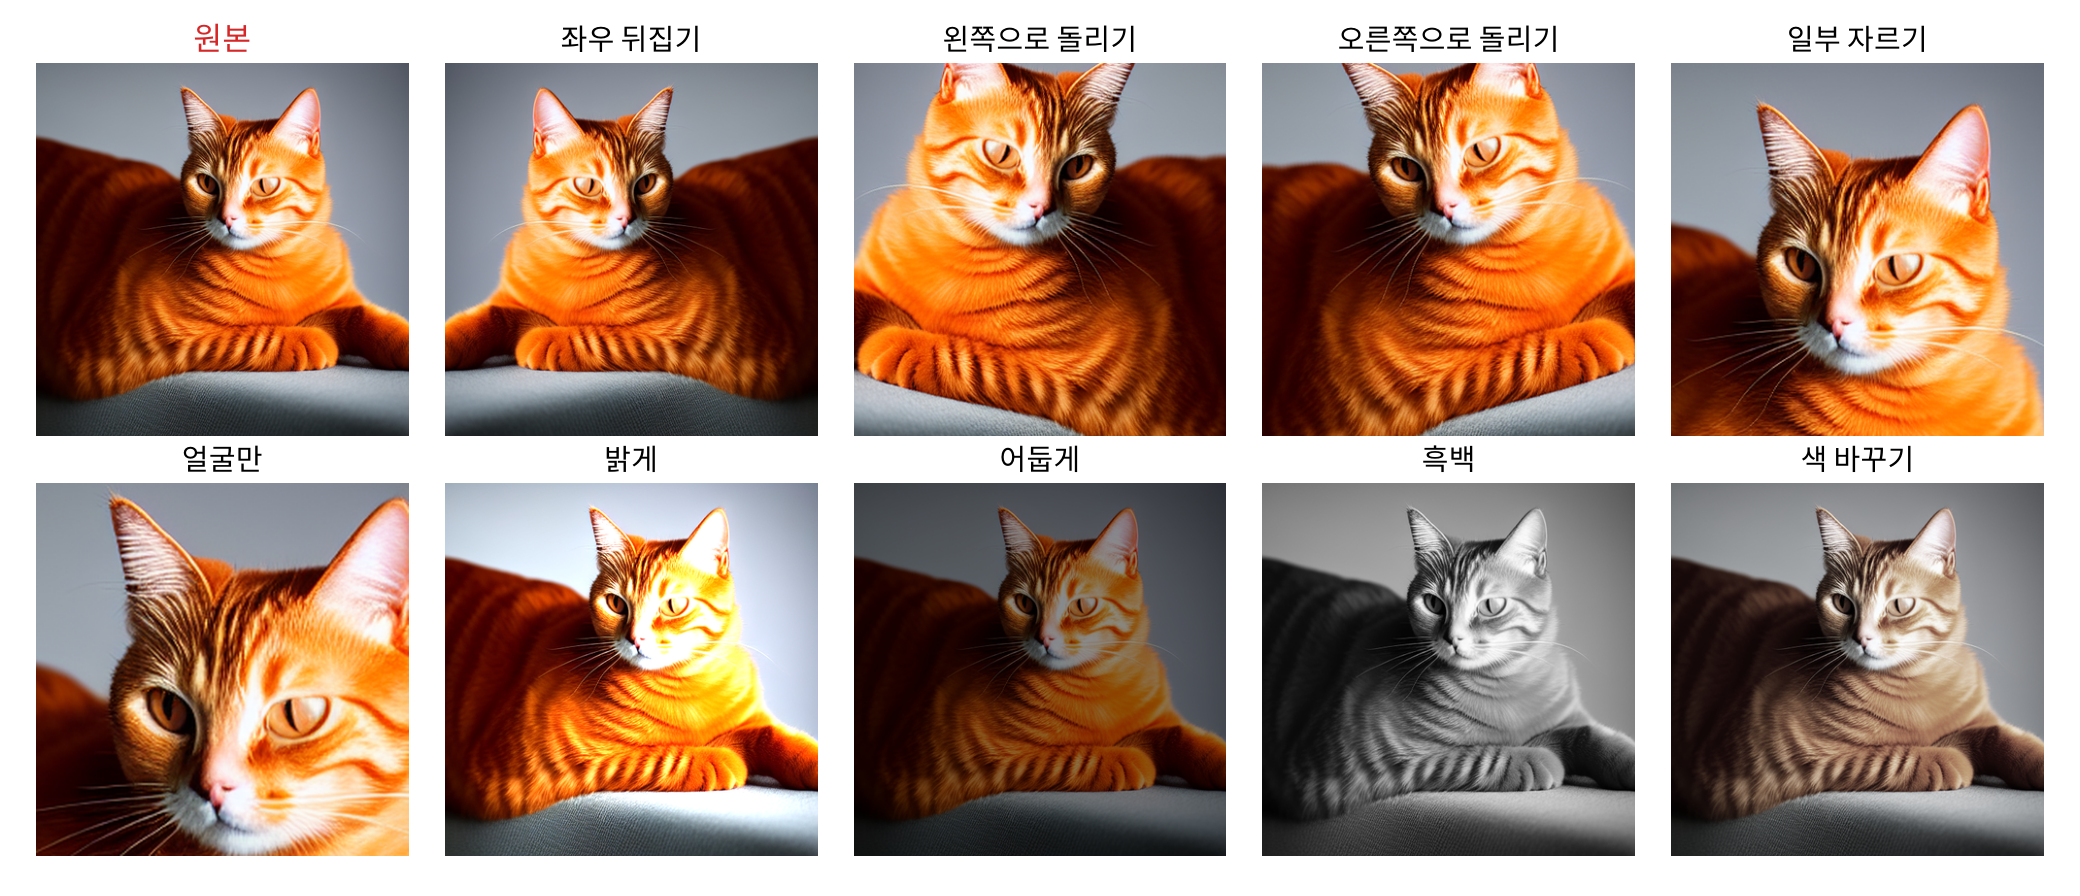
\includegraphics[width=0.9\linewidth]{da_cats.png}\par\vskip0.2em
{\large 사람 눈엔 \kb{모두 같은 고양이} $\to$ 정답도 그대로 ``고양이''}
\vfill
\note{원본 고양이 사진을 좌우로 뒤집고, 왼쪽과 오른쪽으로 살짝 돌리고, 일부를 잘라 내고, 얼굴만 남기고, 밝게, 어둡게, 흑백으로, 색을 바꿔 봤습니다. 사진은 달라졌지만 사람 눈에는 모두 같은 고양이입니다. 그러니 정답도 그대로 고양이라고 붙여 학습 데이터로 쓸 수 있습니다. 한 장이 열 장이 됐습니다. 참고로 이 고양이 사진은 AI로 생성한 그림입니다.}
\end{frame}

% --- 원리
\begin{frame}{왜 도움이 되나: ``이런 변화는 상관없다''를 가르친다}
\vfill
\centering
{\large 모델은 학습 데이터에 없는 변화를 모른다 (오른쪽 보는 고양이만 봤다면?)}\\[0.8em]
{\Large 증강 = \kb{답을 바꾸지 않는 변화}를 데이터로 알려 주기}\\[0.8em]
{\large 뒤집어도 · 돌려도 · 밝기가 달라도 고양이 $\to$ 그 변화를 \textbf{무시하는 법}을 배운다}\\[0.4em]
{\small 사람이 아는 사실 (불변성) 을 데이터로 넣어 주는 셈 \quad 과대적합도 줄어든다 (같은 사진을 외우기 어렵다)}
\vfill
\note{왜 도움이 될까요? 모델은 학습 데이터에 없는 변화를 모릅니다. 오른쪽을 보는 고양이 사진만 본 모델은 왼쪽을 보는 고양이를 못 알아볼 수 있습니다. 데이터 증강은 답을 바꾸지 않는 변화를 데이터로 알려 주는 방법입니다. 뒤집어도, 조금 돌려도, 밝기가 달라도 고양이라는 걸 보여 주면, 모델은 그런 변화를 무시하는 법을 배웁니다. 사람이 이미 아는 사실을 데이터로 넣어 주는 셈입니다. 또 매번 조금씩 다른 사진을 보니 같은 사진을 그대로 외우기 어려워서 과대적합도 줄어듭니다.}
\end{frame}

% --- 숫자 증강
\begin{frame}{실험: 손글씨 숫자 100장으로}
\vfill
\centering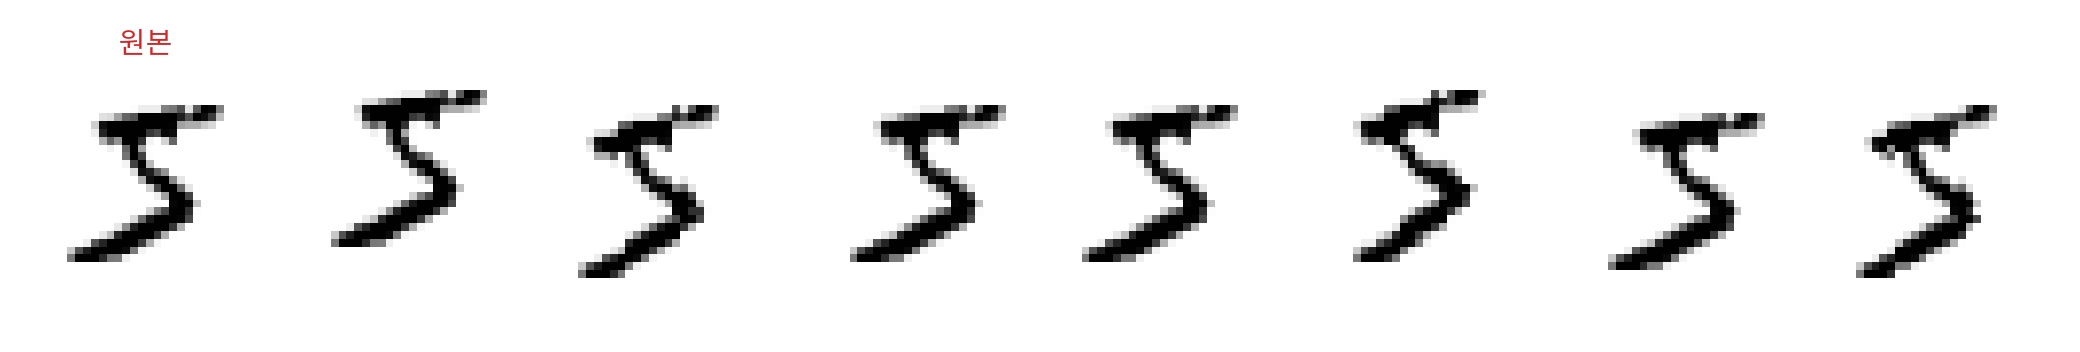
\includegraphics[width=0.86\linewidth]{da_digits.png}\par\vskip0.4em
{\large 숫자마다 \textbf{10장씩, 모두 100장}만으로 작은 CNN 을 학습 (400 에폭)}\\[0.4em]
{\large 증강: 매 에폭 \textbf{무작위로} $\pm 10$ 도 돌리고 $\pm 2$ 칸 밀기}
\vfill
\note{실제로 실험해 봤습니다. 손글씨 숫자를 숫자마다 10장씩, 모두 100장만 써서 작은 CNN을 학습했습니다. 데이터가 아주 적은 상황입니다. 증강은 매 에폭마다 그림을 무작위로 10도 이내에서 돌리고, 2칸 이내에서 상하좌우로 밀었습니다. 위 그림은 숫자 5 한 장을 이렇게 바꾼 예입니다. 같은 100장이지만 모델은 매번 조금씩 다른 그림을 보게 됩니다.}
\end{frame}

% --- 결과
\begin{frame}{결과: 78\% $\to$ 87\%}
\markpage{result}
\vfill
\centering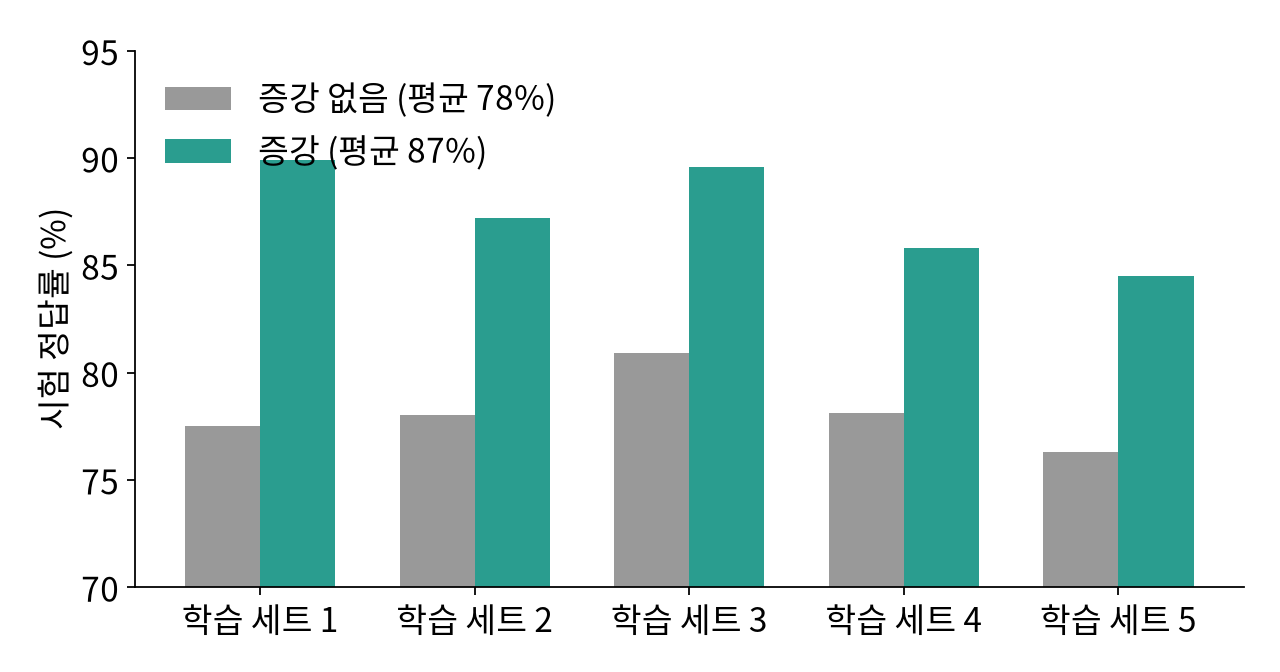
\includegraphics[width=0.56\linewidth]{da_result.png}\par\vskip0.2em
{\large 시험 1만 장: 증강 없음 \textbf{78\%} \quad 증강 \kb{87\%} \quad (학습 세트 5개 모두 증강 승)}\\[0.2em]
{\small 사진을 한 장도 더 모으지 않았다}
\vfill
\note{결과입니다. 시험 1만 장에서 증강 없이는 평균 78퍼센트, 증강을 하면 87퍼센트입니다. 운을 배제하려고 서로 다른 100장 학습 세트 다섯 개로 해 봤는데, 다섯 번 모두 증강 쪽이 이겼습니다. 사진은 한 장도 더 모으지 않았는데 9퍼센트포인트가 올랐습니다.}
\end{frame}

% --- 주의
\begin{frame}{주의: 뜻이 바뀌는 변형은 안 된다}
\vfill
\centering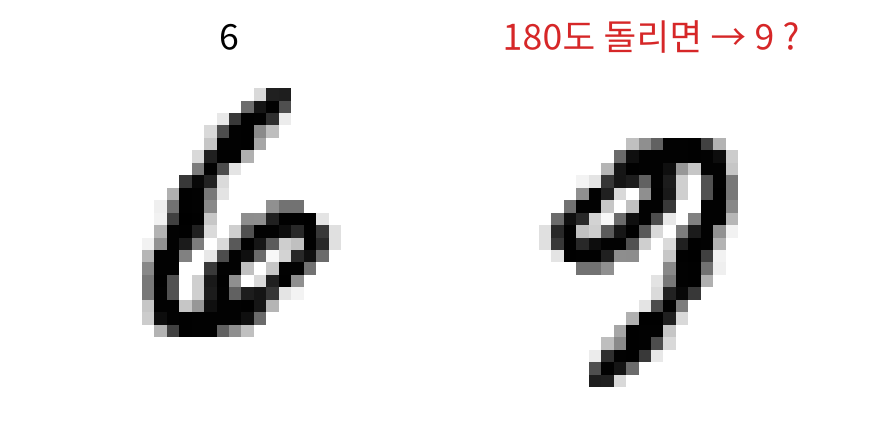
\includegraphics[width=0.36\linewidth]{da_six.png}\par\vskip0.3em
\renewcommand{\arraystretch}{1.4}
{\large\begin{tabular}{ll}
숫자 & 6 을 180도 돌리면 9 \quad 많이 돌리면 \kq{정답이 바뀐다}\\
글자 & b 를 좌우로 뒤집으면 d\\
의료 영상 & 좌우를 뒤집으면 심장이 반대편 \quad 왼쪽 · 오른쪽이 중요한 진단이면 금지\\
위성 사진 & 위아래 뒤집기는 괜찮다 (하늘에서 내려다보니까)
\end{tabular}}\vskip0.4em
{\large 어떤 변화가 \textbf{답을 바꾸지 않는지}는 문제를 아는 사람이 정한다}
\vfill
\note{주의할 점이 있습니다. 뜻이 바뀌는 변형은 쓰면 안 됩니다. 숫자 6을 180도 돌리면 9가 됩니다. 그래서 손글씨에는 10도 정도만 돌렸습니다. 글자 b를 좌우로 뒤집으면 d가 됩니다. 흉부 엑스레이를 좌우로 뒤집으면 심장이 반대편에 있게 되니, 왼쪽 오른쪽이 중요한 진단이라면 뒤집기는 금지입니다. 반대로 위성 사진은 하늘에서 내려다본 것이라 위아래로 뒤집어도 괜찮습니다. 어떤 변화가 답을 바꾸지 않는지는 결국 그 문제를 아는 사람이 정해야 합니다.}
\end{frame}

% --- AlexNet
\begin{frame}{AlexNet (2012) 도 증강으로 2048배}
\vfill
\centering
{\large 256 × 256 사진에서 224 × 224 조각을 위치를 바꿔 가며 잘라 내고 \quad + 좌우 뒤집기}\vskip0.6em
{\LARGE\[ \underbrace{(256 - 224) \times (256 - 224)}_{\text{위치 1,024 가지}} \times \underbrace{2}_{\text{뒤집기}} = \kb{2{,}048} \]}\vskip0.2em
{\large 논문: 증강이 없으면 심한 과대적합으로 훨씬 작은 신경망을 써야 했을 것}\\[0.4em]
{\small Krizhevsky, Sutskever, Hinton (2012) \quad 밝기 · 색을 바꾸는 증강도 함께 썼다}
\vfill
\note{2012년 이미지넷 대회 1위 AlexNet도 데이터 증강을 썼습니다. 256 곱하기 256 사진에서 224 곱하기 224 조각을 위치를 바꿔 가며 잘라 내면 32 곱하기 32, 1024가지 위치가 나오고, 좌우 뒤집기까지 하면 2048배가 됩니다. 논문은 이 증강이 없었다면 심한 과대적합 때문에 훨씬 작은 신경망을 써야 했을 거라고 썼습니다. 밝기와 색을 바꾸는 증강도 함께 썼습니다. 지난 시간의 드롭아웃과 함께 AlexNet이 과대적합을 막은 두 무기였습니다.}
\end{frame}

% --- 언제
\begin{frame}{언제, 어떻게 적용하나}
\vfill
\centering
\renewcommand{\arraystretch}{1.5}
{\large\begin{tabular}{ll}
\textbf{학습 데이터에만} & 검증 · 시험 데이터는 원본 그대로 (그래야 정직한 평가)\\
\textbf{매 에폭 새로} & 미리 저장하지 않고, 읽을 때마다 무작위로\\
\textbf{분할 먼저} & 증강 전에 나눈다 (같은 사진의 변형이 양쪽에 = 누수)\\
PyTorch & \texttt{transforms.RandomHorizontalFlip}, \texttt{RandomAffine}, \texttt{ColorJitter} $\cdots$
\end{tabular}}
\vfill
\note{적용할 때 지킬 것이 있습니다. 증강은 학습 데이터에만 합니다. 검증과 시험 데이터는 원본 그대로 둬야 정직한 평가가 됩니다. 보통 미리 10배로 만들어 저장하지 않고, 데이터를 읽을 때마다 무작위로 바꿉니다. 그러면 에폭마다 새로운 변형을 봅니다. 그리고 6주차의 누수를 기억하세요. train과 test를 나누기 전에 증강하면 같은 사진의 변형이 양쪽에 들어가 성능이 부풀려집니다. 반드시 나누고 나서 학습 쪽에만 합니다. PyTorch에는 뒤집기, 돌리기, 색 바꾸기 같은 변환이 준비되어 있습니다.}
\end{frame}

% --- 다른 분야
\begin{frame}{그림 말고도}
\vfill
\centering
\renewcommand{\arraystretch}{1.5}
{\large\begin{tabular}{ll}
\textbf{소리} & 속도 · 높이 바꾸기, 배경 잡음 섞기\\
\textbf{글} & 같은 뜻의 단어로, 번역했다가 되돌리기 (back-translation)\\
\textbf{표 데이터} & 조심스럽다: 숫자를 바꾸면 뜻이 바뀌기 쉽다\\
\textbf{섞기} & 두 사진과 정답을 비율대로 섞기 (mixup, CutMix)
\end{tabular}}\vskip0.8em
{\large 공통 질문: ``\textbf{이렇게 바꿔도 정답이 같은가?}''}
\vfill
\note{증강은 그림 말고도 씁니다. 소리는 속도나 음 높이를 바꾸거나 배경 잡음을 섞습니다. 글은 같은 뜻의 단어로 바꾸거나, 다른 언어로 번역했다가 다시 번역해 되돌리는 방법을 씁니다. 표 데이터는 조심스럽습니다. 혈압 숫자를 바꾸면 진단이 바뀔 수 있으니까요. 두 사진과 정답을 비율대로 섞는 mixup처럼 좀 더 과감한 방법도 있습니다. 어느 분야든 질문은 하나입니다. 이렇게 바꿔도 정답이 같은가.}
\end{frame}

% --- 문제풀이
\begin{frame}{문제풀이}
\vfill
\begin{enumerate}
\item 다음 중 증강으로 쓰면 \textbf{안 되는} 것을 고르라. (a) 강아지 사진 좌우 뒤집기 \; (b) 숫자 손글씨 90도 돌리기 \; (c) 자동차 사진 밝기 바꾸기 \; (d) 도로 표지판 ``좌회전'' 좌우 뒤집기\vskip0.8em
\item 300 × 300 사진에서 280 × 280 조각을 잘라 내고 좌우 뒤집기까지 하면 몇 배인가?\vskip0.8em
\item 사진 1,000장을 먼저 10배로 증강해 1만 장을 만든 뒤 무작위로 학습 · 시험을 나눴다. 문제는?
\end{enumerate}
\vfill
\note{1번 답. b와 d입니다. 손글씨를 90도 돌리면 다른 글자처럼 보일 수 있고, 6과 9처럼 정답이 바뀌기도 합니다. 좌회전 표지판을 뒤집으면 우회전이 됩니다. 2번 답. 20 곱하기 20, 400가지 위치에 뒤집기 2를 곱해 800배입니다. 3번 답. 같은 사진의 변형이 학습과 시험 양쪽에 들어가는 누수입니다. 먼저 나누고 학습 쪽만 증강해야 합니다.}
\end{frame}

% --- 실습
\begin{frame}{실습}
\vfill
\centering\begin{tabular}{rl}
\large 1 & 직접 만드는 증강: numpy 로 뒤집기 · 밀기 · 밝기, torchvision 변환과 비교\\[0.5em]
\large 2 & 손글씨 100장: 증강 없음 vs 증강 (78\% $\to$ 87\% 재현, 학습 세트 하나)\\[0.5em]
\large 3 & 너무 센 증강 (180도 돌리기) 은 어떻게 되나
\end{tabular}\vskip1em
MNIST (torchvision) \\[0.4em]\href{https://colab.research.google.com/github/SuminHan/book-ml/blob/main/slides/v2/ml1/week10/data_augmentation/lab/data_augmentation.ipynb}{\textcolor{ksagolddk}{▶ Colab에서 실습 노트북 열기}}
\vfill
\note{실습은 세 부분입니다. 첫째, numpy로 뒤집기, 밀기, 밝기 바꾸기를 직접 만들어 보고 torchvision 변환과 비교합니다. 둘째, 손글씨 100장으로 증강이 없을 때와 있을 때를 비교해 오늘의 결과를 재현합니다. 셋째, 180도처럼 너무 센 증강을 쓰면 오히려 어떻게 되는지 확인합니다.}
\end{frame}

% --- 정리
\begin{frame}{정리}
\vfill
\centering\large\begin{tabular}{l}
\textbf{데이터 증강}: 뜻은 그대로, 모양만 바꿔 학습 데이터를 늘린다\\[0.5em]
답을 바꾸지 않는 변화를 가르친다 \quad 과대적합도 줄어든다\\[0.5em]
손글씨 100장: 78\% $\to$ \kb{87\%} \quad AlexNet: 2,048배\\[0.5em]
\kq{뜻이 바뀌는 변형 금지} (6 $\leftrightarrow$ 9) \quad 학습 데이터에만, 분할한 뒤에
\end{tabular}
\vfill
\note{정리합니다. 데이터 증강은 뜻은 그대로 두고 모양만 바꿔 학습 데이터를 늘리는 방법입니다. 답을 바꾸지 않는 변화를 모델에게 가르치고, 과대적합도 줄여 줍니다. 손글씨 100장으로 78퍼센트가 87퍼센트로 올랐고, AlexNet은 2048배로 늘렸습니다. 다만 6과 9처럼 뜻이 바뀌는 변형은 쓰면 안 되고, 학습 데이터에만, 그리고 train과 test를 나눈 뒤에 적용합니다.}
\end{frame}

% --- 이미지 출처
\begin{frame}{이미지 출처}
\vfill
\centering
{\large 고양이 사진 \pref{cats}: AI 생성 이미지 (Stable Diffusion v1.5), 변형은 직접 만듦}\\[0.6em]
{\large 손글씨 숫자: MNIST (LeCun, Cortes, Burges)}
\vfill
\note{이 덱에 쓴 이미지의 출처입니다.}
\end{frame}
\end{document}
